\documentclass[12pt,a4paper]{article}
%====================== PACKAGES ======================

\usepackage[latin1, utf8]{inputenc}
\usepackage[LAE,T1]{fontenc}
\usepackage[francais]{babel}
%Line break after paragraphes 
\usepackage[raggedright]{titlesec}
\titleformat{\paragraph}[hang]{\normalfont\normalsize\bfseries}{\theparagraph}{1em}{}
\titlespacing*{\paragraph}{0pt}{3.25ex plus 1ex minus .2ex}{0.5em}
%Making quotes before parts
\usepackage{epigraph}
%Changing sections 
\usepackage{titlesec}

\titleformat*{\section}{\LARGE\bfseries}
\titleformat*{\subsection}{\Large\bfseries}
\titleformat*{\subsubsection}{\large\bfseries}
\titleformat*{\paragraph}{\large\bfseries}
\titleformat*{\subparagraph}{\large\bfseries}

% Load the package
% Load the package with the acronym option

%Multi colonnes 
\usepackage{multicol}


%Mis en page :
\usepackage{lastpage}
\usepackage[top=2cm, bottom=2cm, left=2cm, right=2cm]{geometry}
\usepackage[Glenn]{fncychap}
\usepackage{fancyvrb}
\usepackage{fancyhdr}
\setlength{\headheight}{13.1pt}

\fancyhead[]{}

\cfoot{}
\fancyfoot[R]{\thepage}
% Redefine the plain page style
\fancypagestyle{plain}{%
	\fancyhead[]{}
 \renewcommand{\headrulewidth}{0pt}
 
	\cfoot{}
	\fancyfoot[R]{\thepage}
}

%Biblio
\usepackage{pdflscape}
\usepackage{afterpage}
\usepackage[authoryear]{natbib}
\usepackage{hyperref}
\hypersetup{
	colorlinks,
	citecolor=blue,
	filecolor=black,
	linkcolor=black,
	urlcolor=black
}

%Page de garde
\usepackage{framed}
%Rotating
\usepackage{rotating}
%\usepackage{tikz}
\newcommand*\rot{\rotatebox{90}}
%Math using equations
\usepackage{amsmath,amsfonts,amssymb}
%pour gérer les positionnement d'images

%caption
\usepackage{caption}
\usepackage[caption=false]{subfig}
\captionsetup[table]{aboveskip=10pt}
\captionsetup[table]{belowskip=10pt}
\captionsetup{justification=centering}
\captionsetup[table]{name=Tableau}
%Toc
%Images and figures
%\usepackage{setspace}
\setlength{\belowcaptionskip}{-10pt}

\usepackage{graphicx}
\graphicspath{ {Resources/} }
\usepackage{float} 
\setlength{\textfloatsep}{1\baselineskip plus 0.2\baselineskip minus 0.8\baselineskip}

%Tables

\setcounter{secnumdepth}{5}
\setcounter{tocdepth}{4}
\usepackage{tabularx}

\usepackage{multirow}
\usepackage{longtable,booktabs}
\usepackage{chngcntr}\counterwithout{figure}{chapter}
\usepackage{chngcntr}\counterwithout{table}{chapter}
\renewcommand{\thetable}{\Roman{table}}


%page de garde
\usepackage{pdfpages}
\hypersetup{							% Information sur le document
	pdfauthor = {KEBAILI Zohra Kaouter,	},			% Auteurs
	pdftitle = {Les anti-patrons linguistiques},			% Titre du document
	pdfsubject = {Rapport},		% Sujet
	pdfkeywords = {Tag1, Tag2, Tag3, ...},	% Mots-clefs
	pdfstartview={FitH}}					% ajuste la page à la largueur de l'écran
\begin{document} 
	%page de garde
	%====================== INCLUSION DES PARTIES ======================
	
\begin{titlepage}
 \begin{center}
 
\includegraphics[scale=0.9]{Others/Resources/entete.png}\\
 \vspace*{1cm}
  \LARGE
  \textbf{Rapport du module Génie logiciel\\}
  \large
 
  \LARGE
  	\vspace{2cm}
  \textbf{Option: Systèmes et ingénierie de logiciels}\\
  \vspace{1cm}
  \LARGE
  \textbf{Thème}\\
  \vspace{1cm}
  \LARGE
  \setlength{\fboxsep}{0.5cm}
  \begin{framed}
	\textbf{Les anti-patrons linguistiques}
  \end{framed}
  \vspace{2cm}
  \begin{table}[H]
   \setlength{\tabcolsep}{2cm}
    \large
	\centering
	\begin{tabular}{ll}
		\textbf{Réalisé par :}    
		 & \textbf{Encadré par : } \\  \\
		 -\textsc{Mlle Kebaili} Zohra Kaouter 
	
	& -\textsc{ Mme Bousbia} Nabila   \\
	

	\end{tabular}
  \end{table}
  \vspace{\fill}
  \large
  \textbf{Promotion 2017/2018}
        
 \end{center}
\end{titlepage}
	\pagenumbering{Roman}
	\pagestyle{fancy}
	\cleardoublepage

	\tableofcontents
	\cleardoublepage

 \newpage
	\chapter*{Liste des sigles et abréviations}% Main chapter title
\begin{table}[H]
	\label{my-label}
	\begin{tabular}{ll}
		\textbf{API} & Application Programming Interface    \\
		\textbf{AST}   & Arbre Syntaxique Abstrait                          \\
		\textbf{CBO}  & Coupling Between Objects                \\
		\textbf{IR}  & Information Retrieval                 \\
		\textbf{LOC}  & Ligne Of Code                     \\
		\textbf{LSI}  & Latent Semantic Indexing                    \\
		\textbf{NL}  & Natural Language               \\
		\textbf{OO} & Orienté Objet \\
			\textbf{RESTful} & REpresentational State Transfer \\
			\textbf{SOA} & Architecture Orientée Service \\
			\textbf{SQL} & Structured Query Language \\
		\textbf{SVM} & Machines à Vecteurs de Support                \\
		
		\textbf{SP}   & Singulier Points                        
	\end{tabular}
\end{table}
	\cleardoublepage

	\listoffigures
	\cleardoublepage
	\pagenumbering{arabic}	
	\chapter*{Introduction générale}
%\section{Introduction}
\tab Avec le développement logiciel continu et rapide, un programme subit beaucoup de changements pendant son cycle de vie, ce qui engendre des fautes suite à des mauvaises habitudes exercées par les développeurs sous préssion ou par ignorance. Ces mauvaises pratiques affecte la qualité logicielle et rend difficile la compréhesion du code que ce soit par l’auteur du code lui même aprés quelques modifications ou bien par d’autres développeurs lors de la maintenance. Cette derniere avec ses types: Corrective, prenventive, adaptive et  perfective, represente une activité enivitable lors du développement logiciel et vise à produire un logiciel de qualité. \\ \tab

Pour améliorer la qualité logicielle, plusieurs techniques existent, parmi ces techniques: l’utilisation de l’information linguistique, l’utilisation des bons identificateurs, la bonne documentation et l’utilisation du bon lexique. C’est pourquoi, de nouveaux travaux de recherches sont apparus pour exploiter l’information linguistique d’un programme pour identifier les mauvaises pratiques liées au coté linguistique d’un programme ce qui a mené à l’apparition des «anti-patrons linguistiques». \\ \tab

L’objectif de ce rapport est de comprendre ce qu’est un anti-patron linguistique, les anti-patrons linguistiques connus jusqu’à maintenant et comment les détecter.


\newpage
\section{Généralités}
Introduction
Une conception parfaite dès le premier coup n’existe pas, ce qui fait de la tâche de conception une tâche itérative. Les concepteurs avec l’expérience ont remarqué qu’il y a quelques chose qui se répètent d’une conception à l’autre , ce qui a donné naissance à la notion de « patron » et « anti patron » de conception .
\section{Généralités sur les patrons de conception}
Ce terme introduit pour la premiere fois par Koenig en 1998, veut dire les mauvaises solutions reccurentes à des probblèmes de systèmes logiciels\cite{brown1998antipatterns}. Il est important pour les développeurs de connaître les anti-patrons pour savoir les situations où une solution peut avoir un impact négatif et donc l’éviter.
Comme les patrons, les anti-patrons ont leur documentation aussi\cite{arnaoudova2010defining}:
\begin{itemize}
\item \textbf{La pseudo-documentation}: donne le nom et le problème de l’anti-patron en question.
\item \textbf{La mini-documentation}:fournit le nom de l’anti-patron, le problème et la solution proposée.
\item \textbf{la documentation complète}:donne le nom le plus connus,d’autres noms s’il en existe,Frequent niveau: à quel niveau cet anti-patrons peut être détécté: niveau application, micro architecture, framework..etc, nom de la solution et son type, les forces déséquilibrées qui ont été sous-estimées comme la gestion de fonctionnalités ou gestion de complextié, la forme génerale de l’anti-patron donnée sous forme de diagramme, symptomes et conséquences, les exceptions connues où cet anti-patron n’a pas d’impact négatif, d’autres anti-patrons liés à l’anti-patron en question, exemple, applicabilité à d’autres niveaux.
\end{itemize}
\\
Les anti-patrons sont dùs à:
\begin{itemize}
\item  La conception sous des contraintes de temps.
\item  Le changement continu du code.
\item Le non-respect des bonnes pratiques de conception et de codage.
\item l’ignorance et/ou la fiérté des developpeurs.
\end{itemize}
\\

L'ensemble des anti-patrons identifiés ont été catégorisés en\cite{brown1998antipatterns}:
\begin{itemize}
\item Anti patrons de développement.
\item Anti patrons de gestion de projet.
\item Anti patrons d’architecture.

   \end{itemize}
\\
Dans la figure \ref{fig:patanti} ci-dessous, \cite{brown1998antipatterns} illusitre la relation entre les patrons et les anti-patrons que ne verrons juste aprés.
\begin{figure}[H]
	\centering
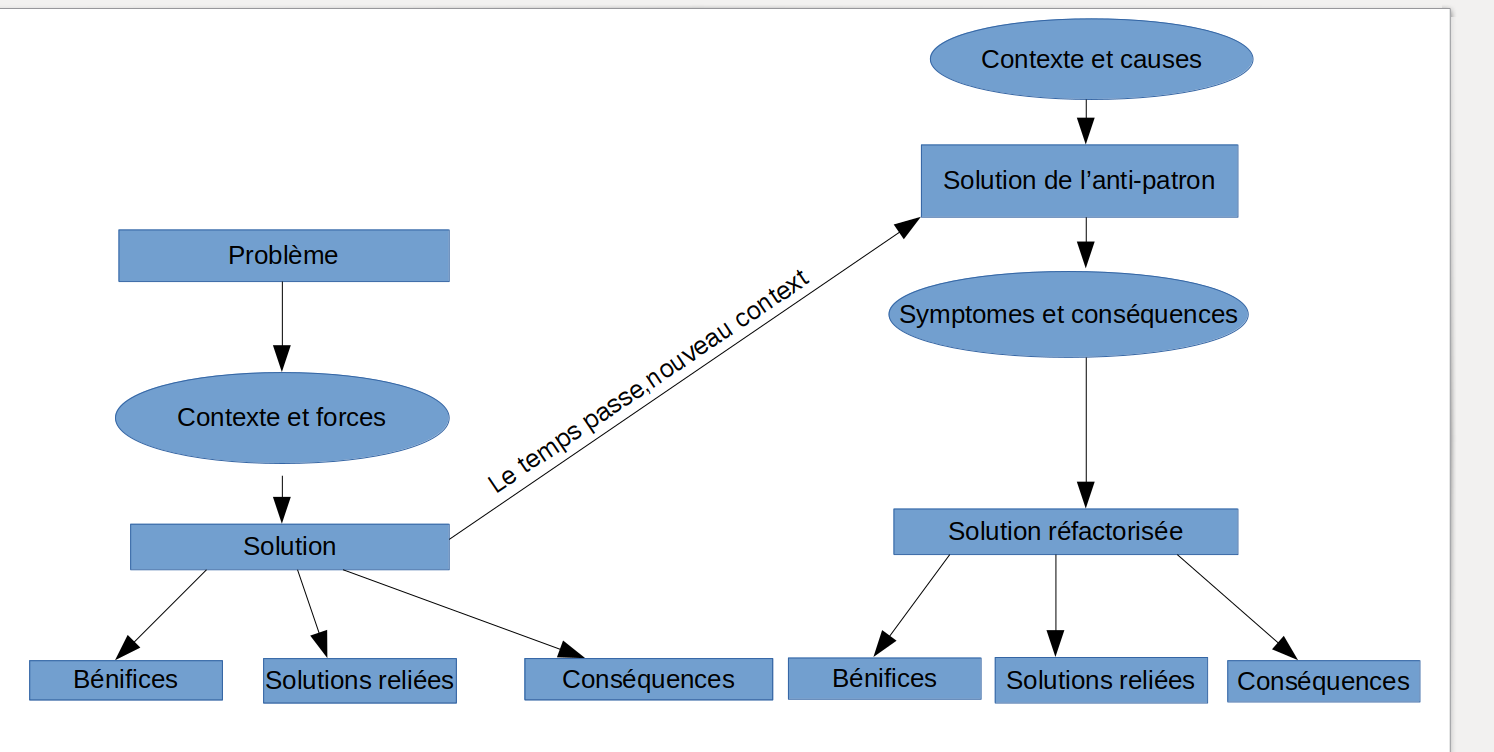
\includegraphics[width=0.9\linewidth]{Others/Resources/patronetantipatron.png}
	\caption{La relation entre les patrons et les anti-patrons \cite{brown1998antipatterns}.}
		\label{fig:patanti}
	\end{figure}
\section{Les anti-Patrons linguistiques}

\label{aplinguistique}
Ils representent une sous-classe des anti-patrons de développement. Ils consistent en les mauvaises habitudes de nomination, de documentation et de choix d’identificateurs  des differentes entités(variables, méthodes, classe-pour les programmes OO...etc) qui reviennent souvent dans les systèmes logiciels qui peuvent affecter la compréhension du code source et/ou la qualité logicielle \cite{brown1998antipatterns}.
L’anti patron linguistique peut etre documenté comme tout autre anti patron, dans ce rapport, nous présentons pour chaque anti-patron linguistique:
\begin{itemize}
\item Son nom
\item Sa description
\item Est ce qu’il concerne une méthode ou un attribut
\item Un exemple tiré d’un vrai programme 
\item Les conséquences possibles de cet anti-patron.
\end{itemize}\\
Puisque nous nous intéressons dans un premier temps, qu’à l’analyse  des attributs et des méthodes dans un code, cette analyse peut être appliquée à d’autres artifacts logiciels comme les diagrammes de classe et les spécifications des APIs.\\

À leurs tours, les anti-patrons linguistiques sont répartis en trois sous-classes à détailler dans le paragraphe suivant pour les méthodes et les attributs \cite{palomba2015anti}:
\begin{itemize}
\item Does more than it says.
\item Says More than it Does
\item Does the Opposite
\end{itemize}
\renewcommand{\thesubsection}{\thesection.\alph{subsection}}
\subsection{Does more than it says}
Ce sont les anti-patrons qui sont détéctés lorsqu’il y a des actions plus que la signature d’une méthode propose \cite{arnaoudova2013new}.

\begin{enumerate}
    

\item \textbf{Plus que des getters} 
\begin{itemize}
\item Description: lorqu’elles fournissent plus que l’attribut concerné en mettant d’autres instructions
\item Appliqué aux: Méthodes
\item Exemple: montré dans la fiqure \ref{fig:un_un} ci-dessous.
	\begin{figure}[H]
	\centering
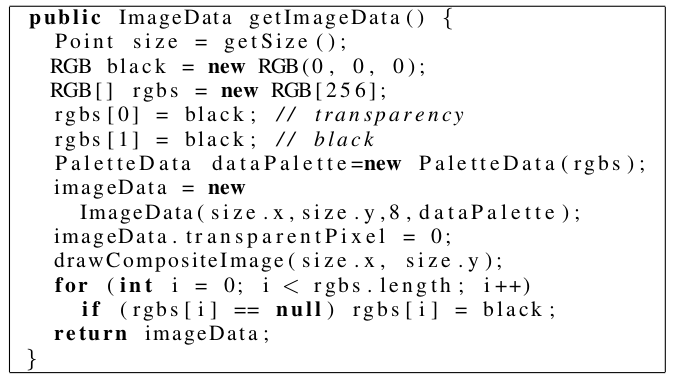
\includegraphics[width=0.9\linewidth]{Others/Resources/un_un.png}
	\caption{Exemple d'un getter qui fait plus que son travail \cite{arnaoudova2013new}.}
		\label{fig:un_un}
	\end{figure}
\item Conséquences: l’utilisation de tels getters engendre l’allocation de nouveaux objets que les getters normallement n’allouent pas.
\end{itemize}
\item \textbf{plus qu’une méthode «is»}
\begin{itemize}
\item Description: Les méthodes qui commencent par “Is” qui sont supposées retourner un booléen mais elles retournent d’autres informations.
\item Appliqué aux: Méthodes
\item Exemple: la figure \ref{fig:un_deux} ilustre un exemple de cet anti-patron.
	\begin{figure}[H]
	\centering
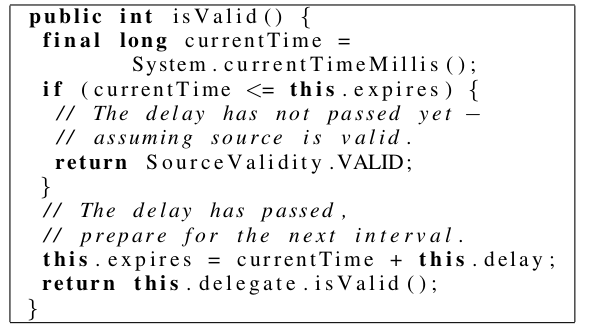
\includegraphics[width=0.9\linewidth]{Others/Resources/un_deux.png}
	\caption{Exemple d'une méthode de type "is" qui fait plus que son travail\cite{arnaoudova2013new}.}
		\label{fig:un_deux}
	\end{figure}
\item Conséquences: une erreur sera déclenchée au moment de la compilation sinon un malentendu de la part des développeurs qui feront la maitenance du programme risque de se produire.
\end{itemize}

\item \textbf{Setter avec retour}
\begin{itemize}

\item Description: Les méthodes setters servent à assigner une valeur à un attribut privé.\\
Ces méthodes ne retournent rien normalement, elles commencent par «set», si un setter se trouve avec une valeur de retour, il doit être renomé.
\item Appliqué aux: Méthodes
\item Exemple: montré dans la figure \ref{fig:un_trois}.
\begin{figure}[H]
	\centering
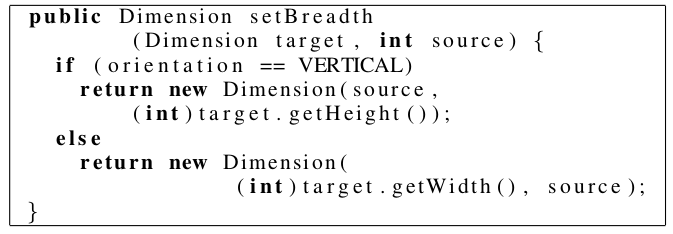
\includegraphics[width=0.9\linewidth]{Others/Resources/un_trois.png}
	\caption{Exemple d'une méthode setter avec retour \cite{arnaoudova2013new}.}
		\label{fig:un_trois}
	\end{figure}
\item Conséquences: il se peut que la méthode setter retourne une valeur liée à un comportement inattendu donc l’erreur ne sera pas captée.

\end{itemize}

\item \textbf{Attendre mais pas recevoir une seule instance}
\begin{itemize}
\item Description: Quand le nom de la méthode fait l’intention de recevoir un seul objet et pas une collection.
Soit une documentation doit être fournie ou bien la méthode doit être renomée.
\item Appliqué aux: Méthodes.
\item Exemple: montré dans la figure \ref{fig:un_quatre}.
\begin{figure}[H]
	\centering
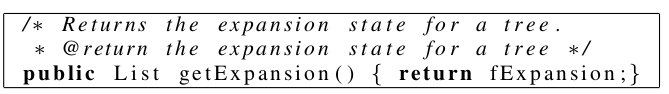
\includegraphics[width=0.9\linewidth]{Others/Resources/un_quatre.png}
	\caption{Exemple de l'anti patron linguistique: Attendre mais pas recevoir une seule instance \cite{arnaoudova2013new}.}
		\label{fig:un_quatre}
	\end{figure}
\item Conséquences: ça ne va pas apparaître au moment de l’execution mais des problèmes de codage pour le développeur, ce dernier va s’attendre à traiter un seul objet, mais il recevra une collection donc, il va être obligé à vériger le corps de la méthode.

\end{itemize}

\end{enumerate}
\subsection{Says More than it Does}
Cet anti-patron apparait lorsqu'une méthode fait mois que ce que la signature d'une méthode propose\cite{arnaoudova2013new}.
\begin{enumerate}
    

\item \textbf {Condition non implémentée}
\begin{itemize}
    \item Description: Quand les commentaires proposent un comportement conditionnel mais le code ne le contient pas.
\item Appliqué aux: Méthodes
\item Exemple: montré dans la figure \ref{fig:deux_un}
\begin{figure}[H]
	\centering
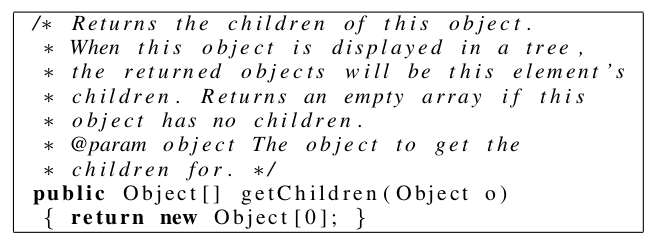
\includegraphics[width=0.9\linewidth]{Others/Resources/deux_un.png}
	\caption{Exemple de l'anti-patron linguistique: Condition non implémentée \cite{{arnaoudova2013new}}.}
		\label{fig:deux_un}
	\end{figure}

\item Conséquences: \\
\begin{enumerate}
    \item La contradiction entre la documentation et le comportement du code va pousser à croire qu’il y a une erreur.
     \item Durant les tests en boite noire, le testeur va inverstir de son temps et effort pour préparer des cas de test selon les differentes conditions mentionnées dans la documentation alors qu’un seul cas pourrait suffir.

\end{enumerate}

\end{itemize}

\item \textbf {Méthode de validation qui ne confirme pas}
\begin{itemize}
\item Description: Une méthode de validation ne retourne pas une valeur pour confirmer cette validation.
\item Appliqué aux: Méthodes
\item Exemple: montré sur la figure \ref{fig:deux_deux}.
\begin{figure}[H]
	\centering
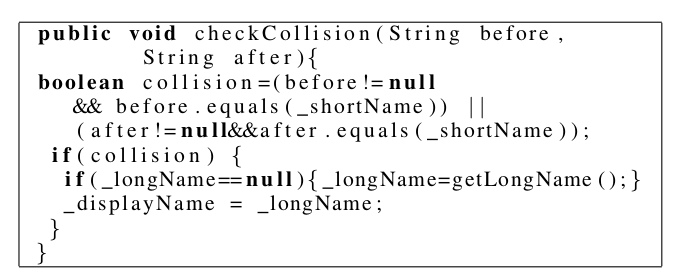
\includegraphics[width=0.9\linewidth]{Others/Resources/deux_deux.png}
	\caption{Exemple d'une méthode de validation qui ne confirme pas\cite{arnaoudova2013new}.}
		\label{fig:deux_deux}
	\end{figure}

\item Conséquences: quelqu’un peut ne pas savoir comment utiliser la sortie de cette méthode, souvent cette sortie est stockée dans une variable quelque part et c’est pas clair au cas d’oubli pour le developpeur ayant écrit cette méthode ou bien au cas de maintenance .
\end{itemize}
\item \textbf{Une méthode getter qui ne retourne rien}
\begin{itemize}
\item Description: le nom de la méthode fait s'attendre à une valeur de retour et ce n’est pas le cas.
\item Appliqué aux: Méthodes.
\item Exemple: montré dans la figure \ref{fig:deux_trois}.
\begin{figure}[H]
	\centering
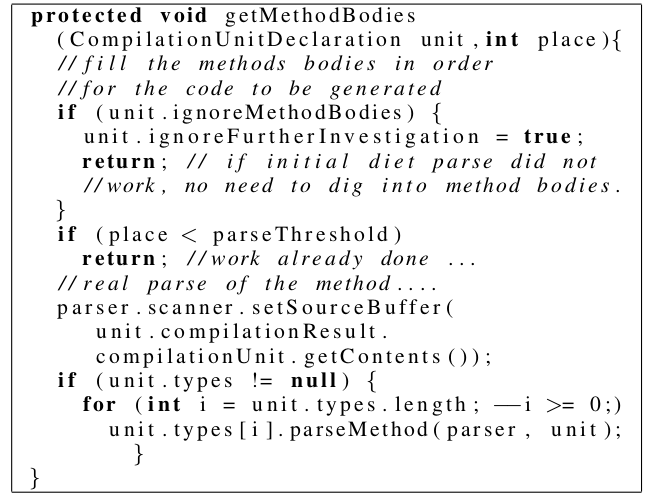
\includegraphics[width=0.9\linewidth]{Others/Resources/deux_trois.png}
	\caption{Exemple d'une méthode getter qui ne retourne rien \cite{arnaoudova2013new}.}
		\label{fig:deux_trois}
	\end{figure}
\item Conséquences: quelqu’un peut assigner la valeur de retour attendue par la méthode getter à une variable et puisque ce n’est pas possible, il va chercher à comprendre le code de la méthode pour trouver la valeur qu’elle fallait retourner.
\end{itemize}

\item \textbf {Question sans réponse}
\begin{itemize}
\item Description: le nom de la méthode commence par «is» ce qui fait s'attendre à un booléen comme valeur retournée mais réellement la méthode ne retourne rien.
\item Appliqué aux: Méthodes.
\item Exemple: montré sur la figure \ref{deux_quatre}.
\begin{figure}[H]
	\centering
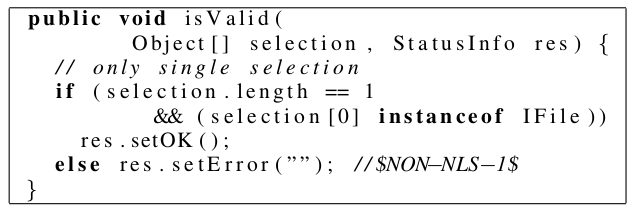
\includegraphics[width=0.9\linewidth]{Others/Resources/deux_quatre.png}
	\caption{Exemple d'une méthode question sans réponse\cite{arnaoudova2013new}.}
		\label{fig:deux_quatre}
	\end{figure}
\item Conséquences: Consequences similaires à celle de “une méthode getter qui ne retourne rien". Dans ce cas ,le développeur va s’attendre à ce qu’il peut utiliser la valeur de retour dans le control d’une condition et ce n’est pas possible car elle ne retourne pas un booléen.
\end{itemize}

\item \textbf {Méthode de transformation sans retour}
\begin{itemize}
\item Description: le nom de la méthode donne l’impression qu’elle transforme un objet mais aucune valeur n’est retournée.
\item Appliqué aux: Méthodes.
\item Exemple: donné dans la figure \ref{fig:deux_cinq}.
\begin{figure}[H]
	\centering
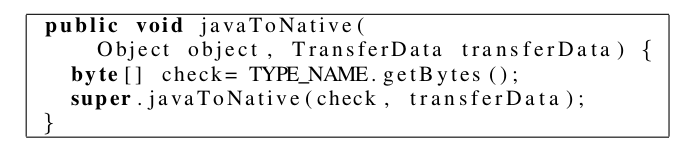
\includegraphics[width=0.9\linewidth]{Others/Resources/deux_cinq.png}
	\caption{Exemple d'une méthode de transformation sans retour\cite{arnaoudova2013new}.}
		\label{fig:deux_cinq}
	\end{figure}
\item Conséquences: Similaire aux précedantes. Ici la valeur de retour pourrait être assignée à une variable dont le nom est inspiré du nom de la méthode.
\end{itemize}

\item \textbf{Attendre une collection mais ne pas la recevoir}
\begin{itemize}
\item Description: Une collection est retournée au lieu d’un seul objet.
\item Appliqué aux: Méthodes.
\item Exemple: montré dans la figure \ref{fig:deux_six}.
\begin{figure}[H]
	\centering

\includegraphics[width=0.9\linewidth]{Others/Resources/deux_six.png}
	\caption{Exemple de l'anti-patrons: Attendre une collection mais ne pas la recevoir\cite{arnaoudova2013new}.}
		\label{fig:deux_six}
	\end{figure}
\item Conséquences: un developpeur peut s’attendre à une collection d’objet et donc il peut utiliser des patrons qui manipulent des collections comme iterator.
\end{itemize}
\end{enumerate}
\subsection{Does the Opposite}
Cet anti-patron apparait dans le cas où il y a une relation d'opposition quelque part dans une méthode\cite{arnaoudova2013new}.
\begin{enumerate}
    

\item \textbf {Le nom de la méthode et le type de retour sont opposés}
\begin{itemize}
\item Description: Ce que veut le nom de la méthode est contradictoire au type de la valeur retournée.
\item Appliqué aux : méthodes.
\item Exemple:montré dans la figure \ref{fig:trois_un}.
\begin{figure}[H]
	\centering
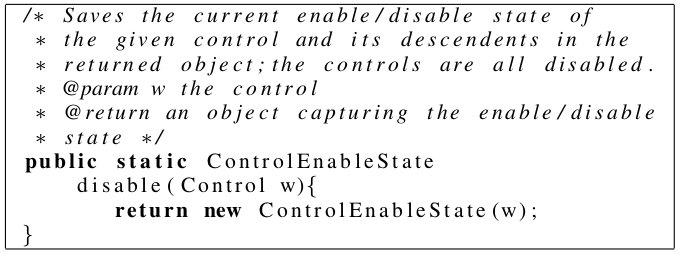
\includegraphics[width=0.9\linewidth]{Others/Resources/trois_un.png}
	\caption{Exemple de l'anti-patrons: Le nom de la méthode et le type de retour sont opposés\cite{arnaoudova2013new}.}
		\label{fig:trois_un}
	\end{figure}
\item Conséquences: les développeurs peuvent se tromper par rapport à la valeur retournée, ça peut ne pas avoir un impact si la méthode retourne un booléen.
\end{itemize}

\item \textbf {La signature de la méthode et les commentaires sont opposés}
\begin{itemize}
\item Description: La documentation de la méthode est contradictoire à sa déclaration(son nom ou bien type retourné).

\item Appliqué aux: Méthodes.
\item Exemple: montré dans la figure \ref{fig:trois_deux}.
\begin{figure}[H]
	\centering
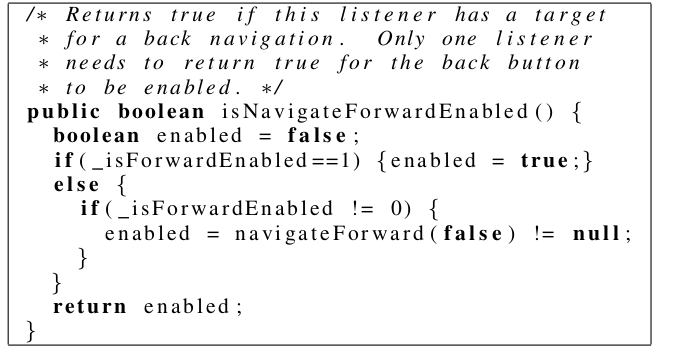
\includegraphics[width=0.9\linewidth]{Others/Resources/trois_deux.png}
	\caption{Exemple de l'anti-patrons:  Signature de la méthode et les commentaires sont opposés\cite{arnaoudova2013new}.}
		\label{fig:trois_deux}
	\end{figure}
\item Conséquences: similaires aux précedantes et peuvent être plus grave car le développeur sera confus, est ce qu’il doit suivre les commentaires ou bien la signature de la méthode, l’un des deux doit étre mis à jour.
\end{itemize}
\end{enumerate}
\subsection{Contains more that it says}
Ce type d'anti-patron concerne les  attributs signifiont plus qu'ils sont réellement \cite{arnaoudova2013new}.
\begin{enumerate}
    

\item \textbf {Dit une chose mais contient beaucoup de choses}
\begin{itemize}
\item Description: Un attribut dont le nom signifie qu’il contient une seule instance mais son type stoque une collection d’objets.
\item Appliqué aux: Attributs.
\item Exemple: montré dans la figure\ref{fig:quatre_un}.
\begin{figure}[H]
	\centering

\includegraphics[width=0.9\linewidth]{Others/Resources/quatre_un.png}
	\caption{Exemple de l'anti-patrons:  Dit une chose mais contient beaucoup de choses\cite{arnaoudova2013new}.}
		\label{fig:quatre_un}
	\end{figure}
\item Conséquences: manque de compréhension de la classe, quand cet attribut change on peut pas savoir l’impact du changement sur les objets manipulés
\end{itemize}

\item \textbf {Nom de booléen mais le type non booléen}
\begin{itemize}

\item Description: Un attribut qui donne l’impression qu’il a deux valeurs soit vraie ou fausse mais sa déclaration est de type  autre que booléen.
\item Appliqué aux: Attributs.
\item Exemple:  comme l’illustre la figure \ref{fig:quatre_deux}
\begin{figure}[H]
	\centering
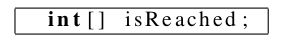
\includegraphics[width=0.9\linewidth]{Others/Resources/quatre_deux.png}
	\caption{Exemple de l'anti-patrons: Nom de booléen mais le type non booléen\cite{arnaoudova2013new}.}
		\label{fig:quatre_deux}
	\end{figure}
\item Conséquence:Le développeur s’attend à ce qu’il soit capable d’utiliser cet attribut dans une instruction de condition mais le type déclaré ne le permet pas .

\end{itemize}
\end{enumerate}
\subsection{Says more than it contains}
Ce type d'anti-patron concerne les  attributs signifiont moins qu'ils sont réellement\cite{arnaoudova2013new}.
\begin{enumerate}
    
\item \textbf {Dit beaucoup de choses mais contient une seule}
\begin{itemize}
\item Description: Un attribut qui donne l’impression du’il contient une collection d’objet mais en réalité il contient un seul objet.
\item Appliqué aux: Attributs.
\item Exemple: montré dans la figure \ref{fig:cinq}
\begin{figure}[H]
	\centering

\includegraphics[width=0.9\linewidth]{Others/Resources/cinq.png}
	\caption{Exemple de l'anti-patrons: Dit beaucoup de choses mais contient une seule\cite{arnaoudova2013new}.}
		\label{fig:cinq}
	\end{figure}
\item Conséquences:manque de compréhesion de l’impact du changement de la l’attribut.
\end{itemize}
\end{enumerate}
\subsection{Contains the opposite}
Ce type d'anti-patron apparait s'il y a une contradition entre un attribut et les commentaires \cite{arnaoudova2013new}.
\begin{enumerate}
    

\item \textbf{L’attribut et son type sont opposés}
\begin{itemize}
\item Appliqué aux: Attributs.
\item Exémple: montré sur la figure \ref{fig:six_un}
\begin{figure}[H]
	\centering
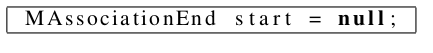
\includegraphics[width=0.9\linewidth]{Others/Resources/six_un.png}
	\caption{Exemple de l'anti-patrons: L’attribut et son type sont opposés\cite{arnaoudova2013new}.}
		\label{fig:six_un}
	\end{figure}
\item Conséquences: ça peut mener à des malentendus, par exemple
un booléen contient l’information qui peut être directlement utilisée dans une condition mais on risque d’inverser les blocs de si sinon.
\end{itemize}
\item \textbf{La signature de l’attribut et le commentaire sont opposés}
\begin{itemize}
\item Description: La docmentation de l’attribut peut être contradictoire au nom ou type de cet attribut.
\item Appliqué aux: Attributs
\item Exemple: montré dans la figure \ref{fig:six_deux}
\begin{figure}[H]
	\centering
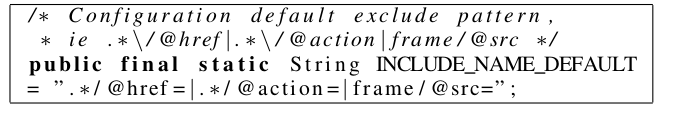
\includegraphics[width=0.9\linewidth]{Others/Resources/six_deux.png}
	\caption{Exemple de l'anti-patrons: La signature de l’attribt et le commentaire sont opposés\cite{arnaoudova2013new}.}
		\label{fig:six_deux}
	\end{figure}
\tem Conséquences: sans analyser profédemment le code source,le developpeur peut ne pas comprendre le rôle de l’attribut.
\end{itemize}

\end{enumerate}


\section{La détéction des anti-patrons linguistiques}
toute détéction d’anti-patron doit passer par deux étapes\cite{brown1998antipatterns}:
\begin{itemize}
    

\item Extraire les informations du code source pour identifier les symptomes des mauvais choix
\item Définir les bons algorithmes pour savoir les anti-patrons linguistques correspondants aux symptomes extraites.
\end{itemize}
\textbf{Pourquoi est-il important de détecter les anti-patrons linguistiques?}\\
Les identificateurs mal choisis augmentent l’effort de comprésension du code source, ces identificateurs peuvent être des mots du dictionnaire, acronyme, ou de simples chaines de caracteres.
L’utilisation des termes identiques dans differents contextes peut augmeter le risque d’apparition de fautes. Cette information prouvée en utilisant deux métriques:l’entropie d’un terme et la couverture d’un contexte par un terme,le but est de montrer que le choix de certains termes augmente la prédisposition aux fautes.Deux métriques sont exploitées à ce niveaux:
\begin{itemize}
    

\item L’entropie d'un terme:  mesure la dispersion physique qui est  le degrés auquel un terme est éparpillé à travers les identificateurs des differentes entités\cite{arnaoudova2010defining}.
\item La couverture d’un context: mesure la dispersion conceptuelle qui est la relation entre ces entités\cite{arnaoudova2010defining}.
\end{itemize}
Si ces deux mesures sont élevées ça veut dire que les termes qui sont beaucoup éparpillés dans le programme  sont utilisés dans des entités non reliées l’une à l’autre  ce qui augmente le risque de prédisposition aux fautes.\\

La détéction des anti-patrons linguistiques est reliée à des domaines\cite{arnaoudova2016linguistic}:
\begin{enumerate}


\item L’entropie et les métriques basées sur la récupération de l’information (information retrieval -based metrics):\\ Plusieurs métriques basées sur l’entropie existent, elles peuvent être appliquées pour expliquer les changements qu’une classe subit à travers plusieurs versions, utilisées pour expliquer la cohesion d’un composant, les méthodes de  la récupération de l’information sont utilisées aussi pour mesurer la qualité d’un code , par exemple, elle servent à mesurer la complexité d’un programme orienté objet, les SVMs et Latent Semantic Indexing(LSI) sont utilisés pour mesurer la cohesion d’une classe, les SVMs sont appliqués pour extraire les identificateurs des entités d’un part, et les identificateurs des commentaires, comparer entre eux, la similarité entre eux indique des entités de bonne qualité.
\item Métriques et prédisposition aux fautes:\\
Ce sont les recherches qui ont pour but de trouver les bonnes métriques comme LOC et CBO qui prédictent le mieux les fautes en calculant la correlation entre ces métriques et la prédisposition aux fautes.
\item L’information linguistique d’un code source:\\
Concerne les recherches de langues essentiellement comme l’ambiguité lexicale, le refactoring stratégique des identificateurs du code source basé sur le lexique standard, d’autres recherches dans ce domaine ont montré que les programmes commentés sont mieux compris par rapportt aux programmes non commentés,les programmes contenant des identificateurs à mots complets sont mieux compris par rapport aux programmes qui contiennent des identificateurs à mots incomplets.
\item Traitement du langage naturel:\\
Ce domaine s’interessent à trouver et mesurer les differents types d’ambiguité(lexicale, syntaxique…) dans le langage naturel, à cause de cette ambiguité, une expression peut être comprise de deux maniere differentes.
\end{enumerate}
\\
\newline
Dans le paragraphe suivant, nous détaillons la détection des anti-patrons linguistiques citées dans la section \ref{aplinguistique}\cite{arnaoudova2016linguistic}:\\
\renewcommand{\thesubsection}{\thesection.\alph{subsection}}
\subsection{Détection des anti-patrons linguistiques de type "Does more than it says"}
\begin{enumerate}
    

\item \textbf{Plus que des getters}\\
Trouver les getters, qui sont les méthodes qui commencent par « get » et se terminent par une chaine de caractères qui correspond à un attribut de meme classe,le type de cet attribut et le type de la valeur retournée par le getter doivent etre les memes. Ensuite,identifier les getters qui fournissent des actions autres que retourner une valeur d’attribut. Des cas où l’attribut est mis à jour avant qu’il soit retourné ne sont pas pris en compte, comme le patron proxy et singleton.
Pour une détection basée sur les expressions du sommet de l’arbre syntaxique abstrait( AST)  autres que l’intruction return est permise sauf dans le cas où un fils d’un control de condition pour la valeur nulle. Autres mesures de complexité comme LOC  ou la compléxité cyclomatique de McCabe peuvent etre utilisés pour une détection simple mais moins exacte.
\item \textbf{plus qu’une méthode «is»}\\
Trouver les méthodes qui commencent par «is» dont le type de retour 
\item \textbf{Setter avec retour}\\
Trouver les méthodes qui commencent par « set » dont le type de retour est different de void.
\item \textbf{Attendre mais pas recevoir une seule instance}\\
Trouver les méthodes qui retournent une collection ( vecteur,tableau…) dont le nom se terminent par un nom en singulier et qui ne contient pas un mot qui signifie une collection.
\end{enumerate}
\subsection{Détection des anti-patrons linguistiques de type "Says More than it Does"}
\begin{enumerate}
\item \textbf{Condition non implémentée}\\
Trouver les méthodes contenant au moins une phrase conditionnelle dans les commentaires, sans qu’il y a des intructions de conditions dans le code.
\item \textbf{Méthode de validation qui ne confirme pas}\\
Trouver les méthodes de validation dont le nom commence par « validate »,check, ensure...etc où le type de retour est void ,sans qu’il y a les instructions d’exception.
\item \textbf{Une méthode getter qui ne retourne rien}\\
Trouver les méthodes dont le nom donne l’impression qu’il y a une valeur de retour mais dont le type de retour est void.
\item \textbf {Question sans réponse}\\
Trouver les méthodes dont le nom commencent par : is ou has, ie, il donne l’impression d’une question,mais le type de retour est void.
\item \textbf{Méthode de transformation sans retour}\\
Trouver les méthode dont le nom propose une transformation, exemple : toString,list2array...etc mais le type de retour est void.
\item \textbf{Attendre une collection mais ne pas la recevoir}\\
Trouver les méthodes don le nom  donne l’impression qu ‘elle retourne un collection,par exemple, qui commence par «get», «return»…,mais le type de retour n’est pas une collection.
\end{enumerate}

\subsection{Détection des anti-patrons linguistiques de type "Does the Opposite"}
\begin{enumerate}
\item \textbf{Le nom de la méthode et le type de retour sont opposés}\\
Trouver les méthodes dont le nom et le type de retour sont des acronoymes.
 \iextbf{La signature de la méthode et les commentaires sont opposé}\\
Trouver les méthode dont le nom ou le type de retour possede une relation d’acronyme avec son commentaire.
\end{enumerate}
\subsection{Détection des anti-patrons linguistiques de type "Contains more that it says"}
\begin{enumerate}
    \item \textbf{Dit une chose mais contient beaucoup de choses}\\
    Trouver les attributs dont le nom se terminent par un nom singulier mais il est déclaré de type collection.
\item \textbf{Nom de booléen mais le type non booléen}\\
Trouver les attributs dont le nom  commence par  un verbe conjugué au troisieme pronom personnel « is » où « has » par exemple, ou qui se termine par un gérondif mais il est déclaré de type autre que booléen.
\end{enumerate}
\subsection{Détection des anti-patrons linguistiques de type "Says more than it contains"}
\begin{enumerate}
    

\item \textbf{Dit beaucoup de choses mais contient une seule}\\
trouver les attributs contenant un nom au pluriel mais déclaré de type autre que collection.
\subsection{Détection des anti-patrons linguistiques de type "Contains the opposite"}
\end{enumerate}
\begin{enumerate}
    

\item \textbf{L'attribut et son type sont opposés}\\
Trouver les attributs dont le nom et leur type de déclaration sont opposés.
\item \textbf{ La signature de l’attribt et le commentaire sont opposés}
\\Trouver les attributs dont le nom ou bien le type de déclaration possède une relation d’acronyme avec son commentaire.
\end{enumerate}

\section{Implementation d’un outil de  détection des anti-patrons linguistiques}
Pour implémenter un outil de détection automatiques des anti-patrons linguistiques, on procède par des étapes qui sont\cite{arnaoudova2013new}:\\
\begin{enumerate}
    

\item \textbf {Exraction des faits à partir du code source}: En utilisant un outil analyseur(parser) comme srcml tool on génére un arabre d’analyse à l’aide duquel on collecte les elements utiles comme les attributs, les noms des méthodes, les commentaires, la pésence des exceptions et des conditions
\item \textbf {Analyse des identificateurs et des commentaires}:
Cette étape a pour but d’identifier les termes qui composent les identificateurs,d’abord en applicant les heuristiques «camel case» et «under score» pour avoir les termes, puis en utilisant l’analyseur de Stanford pour le langage naturel pour savoir si un terme est un nom , adjective ou adverbe...etc,savoir si un nom est au singulier ou au pluriel, la relation entre les mots comme la négation.
\item \textbf{Lier entre les termes des identificateurs et les termes des commentaires}: En utilisant l’outil WordNet ontology, des liaisons de synonymes ou  d’acronymes sont établies.
\end{enumerate}

\section{Les anti-patrons dans les APIs RESTful}
L’architecture SOA est devenue une parmi les plus architecutre adoptées,surtout son style architectural «REpresentational State Transfer» privilégié par beaucoup d’entreprises de production de logiciels comme twitter, facebook et youtube.
Vu que les developpeurs utilisant ces APIs ont besoins de les comprendre pour pouvoir les exploiter dans leurs applications web, c’est pourquoi, les developpeurs tendent vers chercher les APIs dont les URIs (Uniform Resource Identifiers) sont bien conçus et bien \textbf{nommés}.

Les cinq anti-patrons linguistiques  apparus dans les applications REST \cite{palma2015restful}:
\begin{enumerate}
    

\item \textbf{Noms de ressources contextualisés Vs Noms de ressources non-contextualisés}
\begin{itemize}
    

\item {Description}: l’URI doit être contextuel,ie, les nœuds d’une URI doivent etre sémantiquement reliés au même contexte.Cet anti-patron apparaît si les nœuds d’une URI n’appartient pas sémantiquement au même contexte.
\item Exemple: \\
https://www.example.com/newspapers/players?id=123  est faux mais \\
https://www.example.com/newspapers/media/page?id=123 est correct.
\item Conséquences:\\
Les noms des ressources non-contextualisés ne fournissent pas un contexte clair pour les requêtes qui dégrade la compréhension des URIs de la part des développeurs qui les utilisent.
\end{itemize}

\item \textbf{Noeuds hiérarchiques vs nœuds non-hiérarchiques}
\begin{itemize}
    

\item Description: chaque nœud composant d’une URI doit être hiérarchiquement relié aux nœuds voisins, donc cet anti-patrons apparaît si on trouve des nœuds dans une URI qui ne sont pas hiérarchiquement reliés  à leurs nœuds voisins.
\item Exemple:\\
https://www.example.com/professors/university/faculty/ est faux mais\\ https://www.example.com/university/faculty/professors/ est correct.
\item Conséquences: ça peur induire à une confusion à propos de l’utilité de l’URI et donc son utilisabilité.
\end{itemize}
\item \textbf{URI propre vs URI amorphe}
\begin{itemize}
    

\item Description: Une URI propre est une URI lisible,dont les noms sont minuscules, sans underscore, sans extensions et sans aucun symbole pouvant compliquer la lecture de l’URI sinon cet anti-patron est identifié.
\item Exemple:\\
https://w\itemww.example.com/NEW Customer/ photo01.jpg/ est faux mais \\
https://www.example.com/customers/1234 est correct.
\item Conséquences: Les mots en lettres majuscules et en lettres minuscules ne signifient pas la même ressource,et en général ça peut mener vers une ambguité dans l'écriture de la requête.
\end{itemize}
\item \textbf{URI sans verbes vs une URI CRUDy}
\begin{itemize}
    

\item Description: Cet anti-patrons apparaît si les méthodes HTTPs : GET, PUT, POST,DELETE sont utilisés dans des URIs contenant des verbes comme create, update..etc
\item exemple:\\
POST https://www.example.com/update/players/age?id=123 est faux\\
mais POST https://www.example.com/players/age?id=123 est correct.
\item Conséquences:
Cet anti-patron cause une confusion, l’utilisateur d’une API risque de surcharger les méthodes http existantes.
\end{itemize}
\item \textbf{Noeuds singularisés vs Noeuds pluralisés}
\begin{itemize}
    

\item Description: Cet anti-patron apparaît si dans les requêtes put/delete, le dernier est au pluriel ou si dans les requêtes post le dernier nœud est au singulier
\item Exemple:\\
DELETE https://www.example.com/team/players \\
 POST https://www.example.com/team/player sont faux mais \\
DELETE https://www.example.com/team/player \\
 POST https://www.example.com/team/players sont corrects.
\item Conséquences:
Si un nœud pluriel est utilisé à la fin d’une URI de requête PUT/DELETE, le client de l’API ne peut pas créer/supprimer une colection de ressources qui peut causer la reponse serveur « 403 forbidden » et même si la reponse est filtrée,le client de l’API peut tomber dans la confusion entre est ce que le contenu accessible/supprimé est une ressource ou plusieurs ressources.
\end{itemize}
\end{enumerate}
La figure ci-dessous \ref{fig:algocontextualise} illustre l’algorithme de détection de l’anti-patrons « noms de ressources non-contextualisé» dans les applications RESTful \cite{palma2015restful}:
\begin{figure}[H]
	\centering
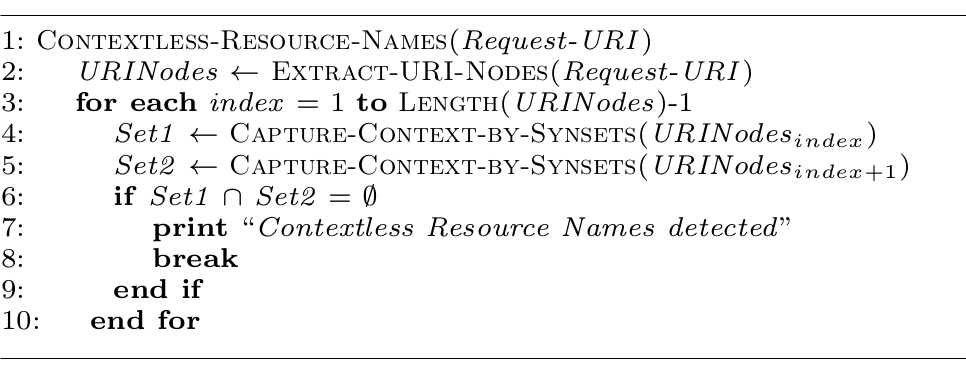
\includegraphics[width=0.9\linewidth]{Others/Resources/algocontextualis.png}
	\caption{L'algorithme de détection de l'anti-patron linguistique noms de ressources non contextualisés \cite{{arnaoudova2013new}}.}
		\label{fig:algocontextualise}
	\end{figure}

L’algorithme procède comme suit :
\begin{itemize}
\item On compare chaque pair de nœud dans une URI 
\item Si on trouve au moins une relation de non-contextualisation
\item Alors l’anti-patron de nom de ressources non-contextualisé.
\end{itemize}
L’ontology WordNet et Stanford CoreNLP pour capter les contextes et effectuer l’analyse sémantique \cite{palma2015restful}.
\\
\cite{palma2015restful} implémentent une solution qui s'appelle "DOLAR"(voir la figure \ref{dolar}) qui détecte les anti-patrons linguistiques dans les applications RESTful, l'article contient les détails de l'implémentation aisni que les résultats de ses tests.
\begin{figure}[H]
	\centering
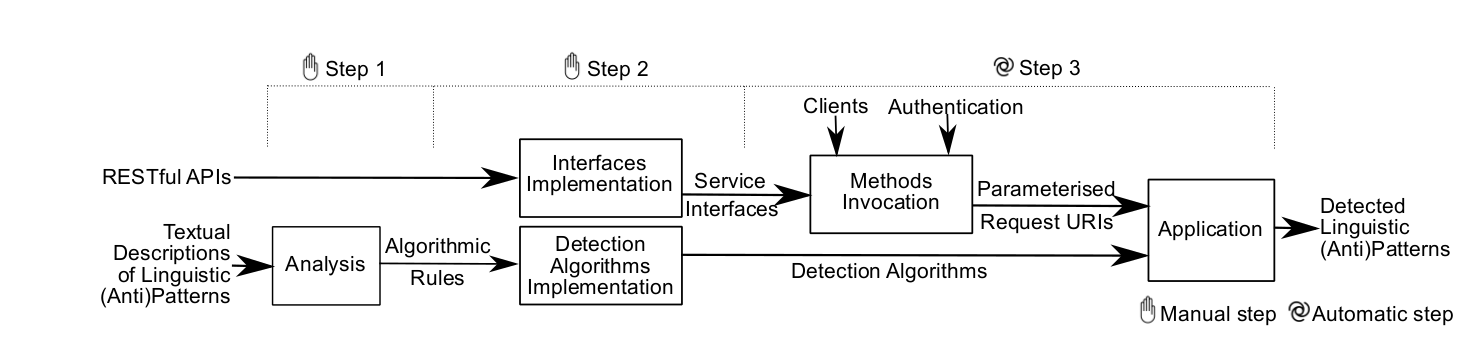
\includegraphics[width=0.9\linewidth]{Others/Resources/dolarapproach.png}
	\caption{L'approche DOLAR \cite{{arnaoudova2013new}}.}
		\label{fig:dolar}
	\end{figure}
\newpage
\section{Conclusion}
\tab Dans ce rapport, nous avons abordé le sujet des anti-patrons linguistiques comme axe de recherches récent dans le domaine de la détection des patrons et des anti-patrons en général. \\ \tab

Cet axe n’est pas encore bien exploité, chose observée pendant la recherches bibliographique, les informations linguistiques ne sont pas toutes exploitées et  peu sont les algorithmes de détection, par exemple l'article \cite{karwin2010sql} propose quelques anti-patrons pour le langage SQL mais les anti-patrons linguistiques SQL ne sont pas invoqués.
\\


\tab Comme synthèse, nous avons établi la liaison entres l’information linguistique,et ses differents métriques et un bon code source,nous avons aussi  touché à l’importance de détéction des anti-patrons linguistiques et leurs solutions refactorisées pour améliorer la qualité logicielle. Il  reste à réaliser un outil pour la détection automatique et exacte des anti-patrons linguistiques avec la possibilité de correction et de refactoring automatique.



	
	%récupérer les citation avec "/footnotemark"
	\nocite{*}
	
	%choix du style de la biblio
	\bibliographystyle{apalike} 
	\renewcommand\bibname{Références}
	\bibliography{bibliographie}

	%voir wiki pour plus d'information sur la syntaxe des entrées d'une bibliographie
	
\end{document}

